% % % % % % % % % % % % % % % % % % % % % % % % % % % % % % % % % % % % % % % %
% LaTeX4EI Template for Cheat Sheets                                Version 1.1
%
% Authors: Emanuel Regnath, Martin Zellner
% Contact: info@latex4ei.de
% Encode: UTF-8, tabwidth = 4, newline = LF
% % % % % % % % % % % % % % % % % % % % % % % % % % % % % % % % % % % % % % % %


% ======================================================================
% Document Settings
% ======================================================================

% possible options: color/nocolor, english/german, threecolumn
% defaults: color, english
\documentclass[eglish/german]{latex4ei/latex4ei_sheet}
\usepackage[ngerman]{babel}
\usepackage{booktabs}
\usepackage{tcolorbox}
% set document information
\title{Cheat Sheet}
\author{RaoulDuke}
\myemail{0x4723@gmail.com}
\mywebsite{www.github.com/doppelplus/CheatSheets}


% ======================================================================
% Begin
% ======================================================================
\begin{document}

\IfFileExists{git.id}{\input{git.id}}{}
\ifdefined\GitRevision\mydate{\GitNiceDate\ (git \GitRevision)}\fi

% Title
% ----------------------------------------------------------------------
\maketitle   % requires ./img/Logo.pdf


% Section
% ----------------------------------------------------------------------
\begin{sectionbox}
	\section{Chemische Grundlagen}
	\subsection{Formelzeichen}
		\begin{tabular}{ll}
			Dichte & $\rho$\\
			Masse & $m$\\
			molare Masse & $M$\\
			Stoffmenge & $n$\\
			Stoffmengenkonzentration & $c$\\
			Volumen & $V$\\
			Liter	& $l$\\
		\end{tabular}

	\subsection{Dichte}
		$ Dichte =  \frac{Masse}{Volumen}$  $ \rho = \frac{m}{V}$
	
	\subsection{Mol und Molare Masse }
		\textbf {Definition atomare Masseneinheit}\\
		$1u = \frac{1}{12}(\ce{^{12}_{6}C}) = 1,66 \cdot 10^{-24}g$\\
		\textbf {Definition Mol}\\
		1 Mol eines Stoffes sind $6,02 \cdot 10^23$ Teilchen dieses Stoffes.\\
		Im PSDE ist die relative Atomasse gleich der Masse eines Mols in g.\\
		\textbf{Beispiel für Molare Masse eines Moleküls}:\\
		Molare Masse von $H_2O$: $M(H_2O) = 2 \cdot M(H)+ M(O) = 2\cdot 1,0\frac{g}{mol} + 16,0\frac{g}{mol}= 18 \frac{g}{mol})$\\
	
	\subsection{Stoffmenge und Konzentration}
		Stoffmenge: $n = \frac{m}{M}$\\
		Stoffemengenkonzentration : $c = \frac{n}{V}$
	\end{sectionbox}

\begin{sectionbox}
	\subsection{Atommodell nach Bohr}
		Hauptschalen entweder 1...8 oder K...R.\\
		Nebenschalen mit maximaler Elektronenanzahl: s(2), p(6), d(10), f(14)\\
		\setlength{\tabcolsep}{0.25em}
		\begin{tabular}{llllllllllllllllllll}
			\ctrule
			1s & 2s & 2p & 3s & 3p & 4s & 3d & 4p & 5s & 4d & 5p & 6s & 4f & 5d & 6p & 7s & 5f & 6d & 7p & 8s\\
			\midrule
			He &  | & Ne &	| & Ar &  | & |  & Kr &  | & |  & Xe &	| &  | & |  & Rn &  |  &  |  &  |  &  $\rightarrow$  &\\
			\ctrule
		\end{tabular}\\
		%Schalenreihenfolge: $\xrightarrow[\text{He \taNe Ar Kr Xe Rn}]{\text{1s 2s 2p 3s 3p 4s 3d 4p 5s 4d 5p 6s 4f 5d 6p 7s 5f 6d 7p 8s}}$\\
	\end{sectionbox}

\begin{sectionbox}
	\subsection{Quantenmechanisches Atommodell}
		\begin{itemize}
			\item Hauptquantenzahl (Hauptschale 1 - 8)$\rightarrow n$
			\item Nebenquantenzahl (Unterschalen 1 - 4 bzw. s - f)$\rightarrow l$
			\item Magnetische Quantenzahl (für 2 $e^-$) $-l$ bis $+l$$\rightarrow m_l$
			\item Magnetische Spinnquantenzahl $m_s \rightarrow \pm \frac{1}{2}$ 
		\end{itemize}
		\vspace{0,5cm}

		{ \fboxsep0.2em
		\begin{tabular}{c|ccc}
			${}_{\color{red}\displaystyle \boldsymbol{n}}\!{\LARGE \diagdown}\!{}^{\color{blue}\displaystyle \boldsymbol{l}}$ & \color{blue}$0 =\textbf{s}$ & \color{blue}$1 = \textbf{p}$ & \color{blue}$2 = \textbf{d}$\\ \mrule
			& $m = 0$ & $m=-1,0,1$ & $m=-2,-1,0,1,2$\\
			\color{red}1:K & \fbox{$\uparrow\downarrow$} & \\[0.2em]
			\color{red}2:L & \fbox{$\uparrow\downarrow$} & \fbox{$\uparrow\downarrow$}\fbox{$\uparrow\downarrow$}\fbox{$\uparrow\downarrow$}\\[0.2em]
			\color{red}3:M & \fbox{$\uparrow\downarrow$} & \fbox{$\uparrow\downarrow$}\fbox{$\uparrow\downarrow$}\fbox{$\uparrow\downarrow$} & \fbox{$\uparrow\downarrow$}\fbox{$\uparrow\downarrow$}\fbox{$\uparrow\downarrow$}\fbox{$\uparrow\downarrow$}\fbox{$\uparrow\downarrow$}\\
			\end{tabular} 
			}
\end{sectionbox}

\begin{sectionbox}
	\textbf{SI-Präfixe}\\
	\begin{tabular}{ccl|ccl}
	Symbol & Vorsatz & Faktor & Symbol & Vorsatz & Faktor \\
	Y&Yotta&$10^{24}$& d &Dezi&$10^{-1}$\\
	Z&Zetta&$10^{21}$& c &Zenti&$10^{-2}$\\
	E&Exa&$10^{18}$& m & Milli&$10^{-3}$\\
	P&Peta&$10^{15}$& $\mu$ & Mikro&$10^{-6}$\\
	T&Tera&$10^{12}$& n &Nano&$10^{-9}$\\
 	G&Giga&$10^9$& p &Piko&$10^{-12}$\\
	M&Mega&$10^6$& f &Femto&$10^{-15}$\\
	k&Kilo&$10^3$& a &Atto&$10^{-18}$\\
	h&Hekto&$10^2$& z & Zepto&$10^{-21}$\\
	da&Deka&$10^1$ & y &Yokto&$10^{-24}$\\
	\end{tabular}
\end{sectionbox}
	\begin{sectionbox}
		\section{Korrosion}
		\begin{itemize}
			\item Ausgangsstoff für chemische Reaktion = Edukt.
			\item Resultierende Verbindung aus Reaktion = Produkt.
			\item Gibbs-Helmholtz-Beziehung: $\Delta G = \Delta H - T\Delta S$.
			\begin{itemize}
				\item Wird Energie frei $\Delta G < 0$ exergonischer Vorgang.
				\item Wird Energie verbraucht $\Delta G>0$, endergonischer Vorgang. 
			\end{itemize}
		\end{itemize}

		\textbf{Regeln zur Bestimmung der Oxidationszahl}
		\begin{itemize}
			\item Im Element ist die Oxidationszahl immer ±0.
			\item Bei einfachen Ionen entspricht die Oxidationszahl immer der Ionenladung.
			\item Die Summe der Oxidationszahlen aller Atome einer Verbindung ergibt die Gesamtladung der Verbindung.
			\item Fluor besitzt in Verbindungen immer die Oxidationszahl –1.
			\item Sauerstoff besitzt in den meisten Fällen die Oxidationszahl –2.
			\item Wasserstoff besitzt in der Regel die Oxidationszahl +1 (Ausnahme: Hydride).
			\item Metalle besitzen in der Regel positive Oxidationszahlen.
			\item Oxidationszahlen anderer Atome in einer Verbindung werden durch Differenzbildung zur Gesamtladung ermittelt.
			\item Bei kovalenten Verbindungen werden die Elektronenpaare dem elektronegativeren Partner zugeordnet.
		\end{itemize}
		
	\end{sectionbox}


		\begin{sectionbox}
			\section{Kunststoffe}
			Bestehen im wesentlichen aus C,H,N und O\\
			\textbf{Polymerisation:} Reaktion von Manomeren mit Doppelbindungen zu makromolekularen Ketten\\[0.5em]
			\textbf{Polykondensation:} Reaktion von Monomere mit reaktiven Endguppen unter Abspaltung von z.B $H_2O$ oder $HCL$\\[0.5em]
			\textbf{Polyaddition:} Venetzung von Epoxiden mit Aminen oder Alkoholen ohne weiteres Reaktionsprodukt\\
			$Polymerisationsgrad = \frac{Molare Masse der Makromolekuele}{Molare Masse der Monomere}$.
			\begin{tabular}{lll}
				\textbf {Typ} & \textbf{Kunststoff} & \textbf{Verwendung}\\
				\midrule
				Thermoplaste & PE(Polyethen) 			& Schläuche\\
							 &				 			& Eimer\\
							 &				 			& Bierkasten\\
							 & PP(Polypropen) 			& Einwegbecher\\
							 &							& Schuhabsätze\\
							 & 							& Flaschen\\
							 & PS(Polystrol)			& Styropor\\
							 &							& Einwegbecher\\
							 &							& Tonbandkassetten\\
							 & PVC(Polyvinylchlorid) 	& Kabelummantelungen\\
							 &							& Duschvorhänge\\
							 &							& Abflussrohre\\
							 & PA(Polyamid)				& Nylonstrümpfe\\
							 &							& Angelschnur\\
							 &							& Brillengestelle\\
				\midrule
				Duroplaste 	 & MF(Phenoplaste)			& Kochlöffel\\
							 & 							& Bakelit\\
							 &							& Küchenmöbeloberflächen\\
							 & UF(Aminoplaste)			& Elektr. Isoliermaterial\\
							 &							& Elektroinstallationen\\
				\midrule
				Elastomere	 & PUR(Polyuretan)			& Matratzen\\
							 &							& Wärmedämmung\\
							 & 							& Kabelummantelungen\\
			\end{tabular}

			
		\end{sectionbox}
		
\begin{sectionbox}
	\section{Moleküle Bindungstypen}
		\begin{tabular*}{\columnwidth}{@{\extracolsep\fill}lll@{}}
		\ctrule
				Bindung & Eigenschaften & Energie \\\cmrule
		Ionisch & Elektronaustausch, stark, starr & $\SI{3.4}{\electronvolt}$ \\
		Kovalent & Gemeinsame Elektronen & \\
		Metallisch & "`Elektronensee"' &  \\
		Dipol & Coulombkräfte von Partialladungen  & \\
		\ctrule
		\end{tabular*}

	\subsubsection{Ionenbindung}
		\underline{Voraussetzung}: unterschiedliche Atome,leicht zu ionisieren
		Je größer die Differenz der Elektronegativitätswerte der beteiligten Atome ist, desto
		stärker ist der ionische Charakter einer Verbindung ausgeprägt.\\
		\begin{itemize}
			\item Coulombanziehung nicht gerichtet $\rightarrow$ positive und negative Ionen lagern so dicht aneinander wie möglich $\rightarrow$ Ionenkristall (nicht verformbar)
			\item Elektronen sind an den Ionen lokalisiert $\rightarrow$ keine freien Elektronen vorhanden $\ra $ Isolator
		\end{itemize}
		Wichtige Anionen:\\
		\begin{tabular}{ll}
			\textbf{Formel} & \textbf{Name}\\
			\midrule
			$SO^{2-}_{4}$ & Sulfat\\
			\midrule
			$SO^{2-}_{3}$ & Sulfit\\
			\midrule
			$HSO^{-}_{4}$ & Hydrogensulfat\\
			\midrule
			$HSO^{-}_{3}$ & Hydrogensulfit\\
			\midrule
			$CO^{2-}_{3}$ & Carbonat\\
			\midrule
			$HCO^{-}_{3}$ & Hydrogencarbonat\\
			\midrule
			$PO^{3-}_{4}$ & Phosphat\\
			\midrule
			$HPO^{2-}_{4}$ & Monohydrogenphosphat\\
			\midrule
			$H_2PO^{2-}_{4}$ & Dihydrogenphosphat\\
			\midrule
			$NO^{-}_{3}$ & Nitrat\\
			\midrule
			$CN^{-}$ & Cyanid.\\
		\end{tabular}\\
	Das Verhältnis von Kationen zu Anionen ist immer derart,
	dass das Molekül elektrisch neutral ist.
		
	\end{sectionbox}

	
	\begin{sectionbox}

		\subsubsection{Kovalente Bindung (Elektronenpaarbindung)}
		Spinabsättigung der äußeren Elektronenschale durch gemeinsame Elektronen
	  
		\begin{itemize}
			\item Valenz-Elektronen zwischen den Atomen lokalisiert
			\item keine Kugelsymmetrische Ladungsverteilung mehr im Atom
			\item Die Anzahl der Elektronen mit umgepaartem Spin zeigt an wie vielfache kovalente Bindungen eingegangen werden können
			\item treten bei und zwischen Elementen der IV. bis VII. Hauptgruppe auf
			\item gerichtete Bindungen $\rightarrow$ mögliche Kristallstrukturen werden eingeschränkt
			\item Differenz der Elektronegativität meist $\Delta E<1.7$
			\item kovalente gebundene Kristalle sind üblicherweise schlechte Leiter 
		\end{itemize}

		\subsubsection{Metallische Bindung}
	Sonderfall der kovalenten Bindung, bei der die Valenz-Elektronen nicht lokalisiert sind.
	\begin{itemize}
    	\item Vorwiegend Elemente mit nur wenigen Außenelektronen
		\item freie Elektronen $\ra $ hohe elektrische Leitfähigkeit, hohe Wärmeleitfähigkeit
		\item Bindung nicht gerichtet $\rightarrow$ hohe Packungsdichte 
		\item Bindungen mit gleich- und ungleichartigen Metallen eingegangen werden
		\item Metallische Bindung ist schwächer als die ionische oder kovalente Bindung
		\item Bindungsstärke hängt von der Zahl der Leitungselektronen ab
	\end{itemize}
	
\subsubsection{Dipolbindung}
	\begin{itemize}
		\item zwischen Molekülen mit permanentem Dipolmoment $\rightarrow$ Moleküle mit positiver und negativer Ladung 
		\item Dipole ordnen sich im Dipolfeld der Nachbaratome so an, dass möglichst geringe Abstand und durch die Coulombkräfte gebunden werden 
    \end{itemize}

\subsubsection{Van-der-Waals-Bindung:} 
        \begin{itemize}
        		\item Atome/Moleküle haben kein permanentes Dipolmoment 
				\item Bindung zwischen Dipolen durch statistische Fluktuationen der Ladungsschwerpunkte.
				\item Sehr schwache Bindung
		\end{itemize}
\subsubsection{Wasserstoffbrückenbindung}
	\underline{Vorraussetzung:} Äußere Schale $>$ vier Elektronen, zwischen 2 Atomen.
		\begin{itemize}
				\item Bindungen über Wasserstoffbrücken der Form A-H-A
				\item Das H-Atom geht eine kovalente Bindung mit Atom der Sorte A ein und gibt sein Elektron ab. Das Proton bleibt fest an Reaktionspartner gebunden und bindet nun zusätzlich das andere negative Atom
				\item Bindungsenergie ist gering $(\SI{0,1}{\electronvolt})$    
 		\end{itemize}
	\end{sectionbox}

	\begin{sectionbox}
		\section{pH-Wert Berechnung}
			Stärke der Base / Säure:\\
			\begin{tabular}{ll}
			$\mathbf{pK_S / pK_A}$ & \textbf{Stärke}\\
			$<-0,35$ & sehr stark\\
			$-0,35 - 0,35 $ & stark bis mittelstark\\
			$>0,35$ & schwach\\
			\end{tabular}\\

			\begin{tabular}{ll}
				starke Säure: & $pH = -\log\cdot c_{S}$\\
				schwache Säure: & $pH = \frac{1}{2}(pK_S-\log\cdot c_{S})$\\
				starke Base: & $pH = 14 - (-\log\cdot c_{B})$\\
				schwache Base: & $pH = 14 - \frac{1}{2}(pK_B-\log\cdot c_{B})$\\
			\end{tabular}

	\end{sectionbox}
\newpage

		\begin{sectionbox}
			\section{Physik}
			\subsection{Formelzeichen}
				\begin{tabular}{lll}
					Größe & Formelzeichen & Einheit\\
					Geschwindigkeit & $v$ & $\frac{m}{s}$\\
					Strecke & $s$ & m\\
					Kraft & $F$ & N(Newton)\\
					Fläche & $A$ & $m^2$\\
					Beschleunigung & $a$ & $\frac{m}{s^2}$.\\
					Drehzahl & $n$ & -\\
					Winkelgeschwindigkeit & $\omega$ & 1/s\\
					Frequenz & $f$ & $Hz$\\
					Periodendauer & T & $\frac{1}{f}$\\
					Arbeit & W & $J$(Joule)\\

				\end{tabular}
			\end{sectionbox}

			\begin{sectionbox}
				\subsection{Bewegungen}
					\textbf{Gleichförmige Bewegung}\\
					$v = \frac{s}{t}$.\\
					\textbf{Gleichmäßig beschleunigte Bewegung und freier Fall}\\
					Beschleunigung: $a = \frac{\Delta v}{\Delta t}$.\\
					Zurückgelegte s bei gleichmäßiger a:
					$s(t)=s_0 + v_0\cdot t+ \frac{a}{2}t^2$\\
					Zurückgelegte Strecke: $ s = \frac{1}{2}\cdot v_{end} \cdot t$\\
					Endgeschwindigkeit : $v_{end}=\sqrt{2 \cdot a \cdot s}$\\
					Endgeschwindigkeit: $v_{end} = v_0 + a \cdot t$\\
					\textbf{Kreisförmige Bewegungen}\\
					Umfangsgeschwindigkeit: $v_u = n \cdot 2 \cdot r \cdot \pi$.\\
					Winkelgeschwindigkeit: $\omega = \frac{\Delta\phi}{\Delta t}$\\
					Radialbeschleunigung: $a_{rad}= 4 \cdot \pi^2 \cdot r \cdot n^2$
			\end{sectionbox}

			\begin{sectionbox}
				\subsection{Kräfte}
				\textbf{Newtonscher Bewegungssatz:}
				\begin{enumerate}
					\item 	Ein Körper verharrt im Zustand der Ruhe oder der gleichförmig geradlinigen Bewegung, sofern er nicht durch einwirkende Kräfte zur Änderung seines Zustands gezwungen wird.
					\item 	Kräfte treten immer paarweise auf. Übt ein Körper A auf einen anderen Körper B eine Kraft aus (actio), 
							so wirkt eine gleich große, aber entgegen gerichtete Kraft von Körper B auf Körper A(reactio)
					\item 	$F = m \cdot a$\\
							$[F] = [m] \cdot [a] = 1 kg \cdot 1\frac{m}{s^2}= 1\frac{kg \cdot m}{s^2} = 1N$.\\
							Ein Newton ist die Kraft, die eine Masse von 1kg die Beschleunigung von $1m/s^2$ verleiht.\\

				\end{enumerate}
				

				$Drehmonment = Kraft \cdot Hebelarm$\\
				Verhältnis aus Kraft zu Hebelarm: $ \frac{F_1}{F_2} = \frac{l_2}{l_1}$.\\

				Reibungszahl: $\mu = \frac{F_R}{F_N}$\\
				
				$F=FH-FR$\\ 
				$m\cdot a=m\cdot g\cdot \sin \alpha-\mu\cdot m\cdot g\cdot \cos \alpha$ und mit $a=\frac{v^2}{2 \cdot }$folgt:\\
				$\mu=\tan \alpha-\frac{v^2}{2\cdot g\cdot \cos \alpha \cdot s}= \mu$\\
				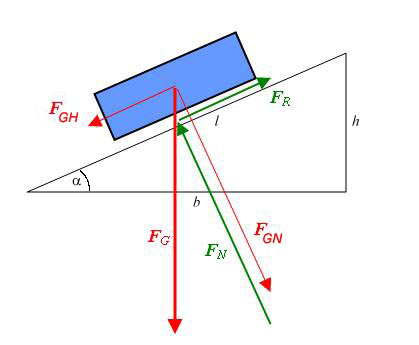
\includegraphics[width=50mm]{img/Schiefe_ebene_4.png}\\

			\end{sectionbox}

			\begin{sectionbox}
				\subsection{Arbeit, Leistung, Wirkungsgrad}
					Ein Joule ist die Arbeit, die aufgebracht werden muss, um eine Kraft von 1 Newton
					entlang eines Weges von 1 Meter wirken zu lassen.\\
					\textbf{Arbeit:} $W= F \cdot s$\\
					\textbf{Hubarbeit:} $W = g \cdot h$ bzw. $W = m \cdot g \cdot h$\\
					\textbf{Reibungsarbeit:} $F_R = \mu \cdot F_N$\\
					\textbf{Arbeit bei schrägem Kraftantrieb:} $W = F \cdot s \cdot \cos \alpha$\\
					\textbf{Beschleunigungsarbeit:} $W = m \cdot a \cdot s$; $W = m \cdot \frac{a^2 \cdot t^2}{2}$; $W = m \cdot \frac{v^2}{2}$\\
					\textbf{Federkonstante:} $c = \frac{F}{s}$\\
					\textbf{Federspannarbeit:} $W = \frac{1}{2}\cdot F \cdot s$; $W = \frac{1}{2}\cdot c \cdot s^2$; $W = \frac{F^2}{2 \cdot c}$\\
					\textbf{potenzielle Energie:} $W_{pot} = m \cdot g \cdot h$\\
					\textbf{kinetische Energie:} $W_{kin} = \frac{1}{2}\cdot m \cdot v^2$\\
					\textbf{Leistung:} $P = \frac{W}{t}$; $P = F \cdot v$\\
					\textbf{Wirkungsgrad:} $\eta = \frac{P_{eff}}{P_{ind}}$, $\eta < 1$\\
					\textbf{Kraftstoß = Impuls:} $F \cdot \Delta t = \Delta v \cdot m$\\
					\textbf{Erhaltung des Impulses:} $m_1 \cdot v_1 + m_2 \cdot v_2 = 0$\\
					
					\textbf{Zentraler elastischer Stoß}\\
					\begin{tabular}{ll}
						\midrule
						kinetische Energie & $m_1 \cdot u_1^2 + m_2 \cdot u_2^2 = m_1 \cdot v_1^2 + m_2 \cdot v_2^2$\\
						Impuls & $m_1 \cdot u_1 + m_2 \cdot u_2 = m_1 \cdot v_1 + m_2 \cdot v_2$\\
						Geschwindigkeiten & $u_1 +v_1 = u_2 + v_2$\\
						v von $m_1$ danach & $v_1 = 2 \cdot \frac{m_1 \cdot u_1 + m_2 \cdot u_2}{m_+ m_2}-u_1 $\\
						v von $m_2$ danach & $v_2 = 2 \cdot \frac{m_1 \cdot u_1 + m_2 \cdot u_2}{m_+ m_2}-u_2  $\\						
						\midrule
					\end{tabular}\\

					\textbf{Zentraler unelastischer Stoß:} $v = \frac{m_1 \cdot v_1 + m_2 \cdot v_2}{m_1+m_2}$\\
					\textbf{Zentripetalkraft:} $F_z = m \cdot a_r$; $F_z = m \cdot \omega^2 \cdot r$; $F_z = \frac{m \cdot v_u^2}{r}$\\
					\textbf{Energie des rotierenden Körpers:} $W_{kin}=\frac{1}{2} \cdot m \cdot r^2 \cdot \omega^2$;  $W_{kin} = I \cdot \frac{\omega^2}{2}$\\
					\textbf{Massenträgheitsmoment:} $I = m \cdot r^2$\\
					\textbf{Massenträgheitsmoment einer rotierenden Scheibe:} $I = \frac{m}{2}\cdot r^2$\\
					
				\end{sectionbox}
				\begin{sectionbox}
				\subsection{Anziehungskräfte}
					\textbf{Anziehung zweier Massen:} $F = \gamma \cdot \frac{m_1 \cdot m_2}{r^2}$\\
					\textbf{Masse eines Himmelskörpers:} $M = \frac{4\pi^2\cdot r^3}{\gamma \cdot T^2}$\\
					\begin{itemize}
						\item M = gesuchte Masse
						\item r = Abstand der beiden Himmelskörper
						\item T = Umlaufdauer des umkreisenden Gestirns
					\end{itemize}

				\end{sectionbox}
				
				\begin{sectionbox}
					\section{Wärmelehre}
						\subsection{Mischen von Flüssigkeiten}
							\subsubsection{Gleiches Material}
								$\vartheta_m = \frac{m_1 \cdot \vartheta_1 + m_2 \cdot \vartheta_2}{m1+m2}$
							\subsubsection{Verschiedene Materialien}
								$\vartheta_m = \frac{C_1 \cdot m_1 \cdot \vartheta_1+C_2 \cdot m_2 \cdot \vartheta_2}{C_1 \cdot m_1 + C_2 \cdot m_2}$
				\end{sectionbox}
\newpage
	\hspace{-5mm}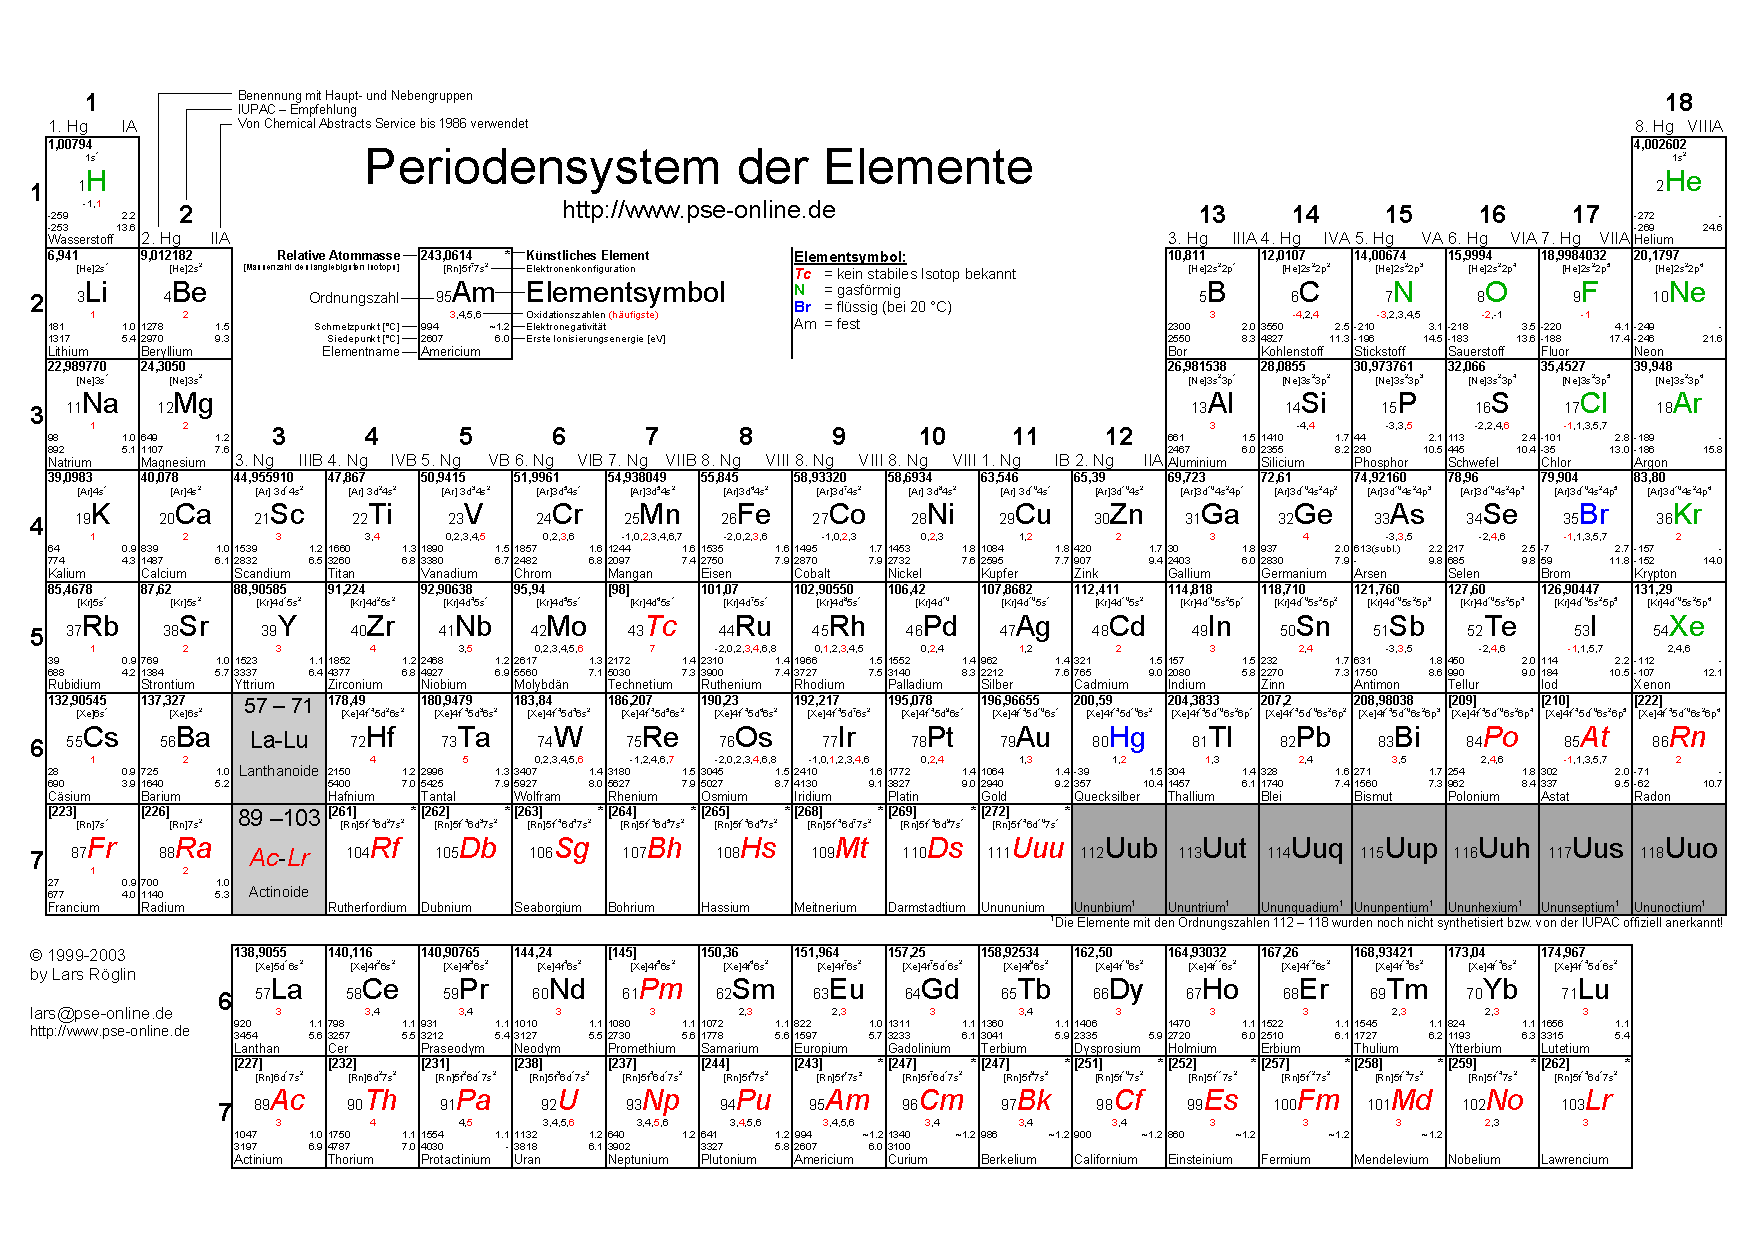
\includegraphics[width = 29.3cm]{img/pse.pdf}
% ======================================================================
% End
% ======================================================================
\end{document}
